%   Filename    : chapter_3.tex 
\chapter{Research Methodology}
This chapter lists and discusses the specific steps and activities performed by the researchers in developing Ha.Zee.

\section{Technologies Used}
The technologies that will be utilized for this project are the following in the following subsections

\subsection{Roboflow}
Roboflow offers a suite  of browser applications to preprocess and preparation of the data for computer vision and machine learning. Roboflow annotation will be used  to manually set bounding boxes for model training and image augmentation for the manipulation of images. \cite{roboflow}

\subsection{Jupyter Notebook using Google Colab and Python}
Jupyter Notebook and Python will be used for training and fitting the data. Jupyter notebook, using google colab,  offers free GPU with CUDA for processing, and Python, the programming language, offers essential libraries for machine learning. \cite{googlecolab}

\subsection{A case  for YOLOv5}
Yolov5 is a pre-trained algorithm that uses a system of grids to detect objects from images or videos (https://docs.ultralytics.com/). This tool will be used for the vehicle detection in this project. 

	YOLOv5 is one of the commonly used algorithm for object detection. It is faster than other object detection algorithms like Region-based Convolutional Neural Networks (RCNN), Fast RCNN, and Faster RCNN. Gandhi \citeyear{gandhi_2018} wrote in an article the comparison between the RCNN algorithms and YOLOv5. He said that the major drawbacks of RCNN are that it classifies 2000 regions per image every time it runs, it cannot run in real time and it is a fixed algorithm. Fast RCNN employs a similar algorithm to RCNN but instead of classifying regions everytime, it uses CNN to generate a convolutional feature map where the bounding regions are derived. Faster RCNN improves upon this by using a different network for predicting the regions of the proposal. In his comparison, he found that Fast RCNN improves on the speed of RCNN significantly. He also mentioned that Faster RCNN, the fastest of the RCNN algorithms, is viable for real-time object detection. 

Aside from the speed of the algorithm, Ultralytics (https://ultralytics.com/) provides extensive documentation of YOLOv5. This is one of the factors that affect the decision of using YOLOv5 for the study.


\section{Research Activities}
To explore YOLOv5 two models will be used. One model is a pre-trained model that comes with YOLOv5 and a custom model trained with a dataset taken from Kaggle. YOLOv5 has options to download and use pre-trained models on the YOLOv5 GitHub page \cite{ultralytics}. This model will serve as a basis to benchmark the performance of the custom data.

\subsection {Data Gathering}
This study plans to identify an area’s pollution level through calculating average of the emissions coming from the cars on the road. In doing so, data of the vehicles, its identification, and its emission rates are needed for the study. Through the use of a camera, a live feed of the vehicles in traffic can be recorded to gather the data of cars in traffic. Image samples of the vehicles (Cars, Motorcycles, and Trucks) will be taken from the Kaggle dataset, Traffic Images Of Vehicles \cite{DVN/POREXF_2020}. This can be utilized in training and testing for the software to recognize the vehicles on the video feed. The vehicle emissions will be taken from an average CO2 emissions of vehicles (four-wheelers and motorcycles) from a dataset provided by Gov.Uk (2020). 

Due to the study being conducted in the country of the Philippines, vehicles such as the local jeepney and tricycle do not have readily available image datasets.Videos and Images of said vehicles in traffic were taken from different angles using a phone camera. 


\subsection {Preprocessing}

	Preprocessing the data includes defining the bounding box of the vehicles in the training data and augmenting the images to make the model perform better. Roboflow has an annotation tool that can be used for  training the model to detect a vehicle in an image and its type. Augmentation of the images will be done by the YOLOv5 algorithm automatically given that the Albumentation library is installed. Augmentation can be used for transforming the images allowing the model to diversify its training data set making it perform better.\cite{dilmegani} 
	

	
\subsubsection{Annotation Method}
Annotation of the vehicles consist of: full image annotation and vehicle cropping. In full image annotation, the entire image or video frame is used and every vehicle present is then selected and categorized for the Roboflow tool to save. Vehicle cropping is when a vehicle/small group of vehicles is/are cropped from the source image/video frame and is then annotated by the tool. This was done when a specific type of vehicle was needed for the database.

Figure \ref{fig:full_img_anno} shows the full image annotation, wherein every bounding box is color coordinated to the type of vehicle used in the study.

\begin{figure}[h!]
	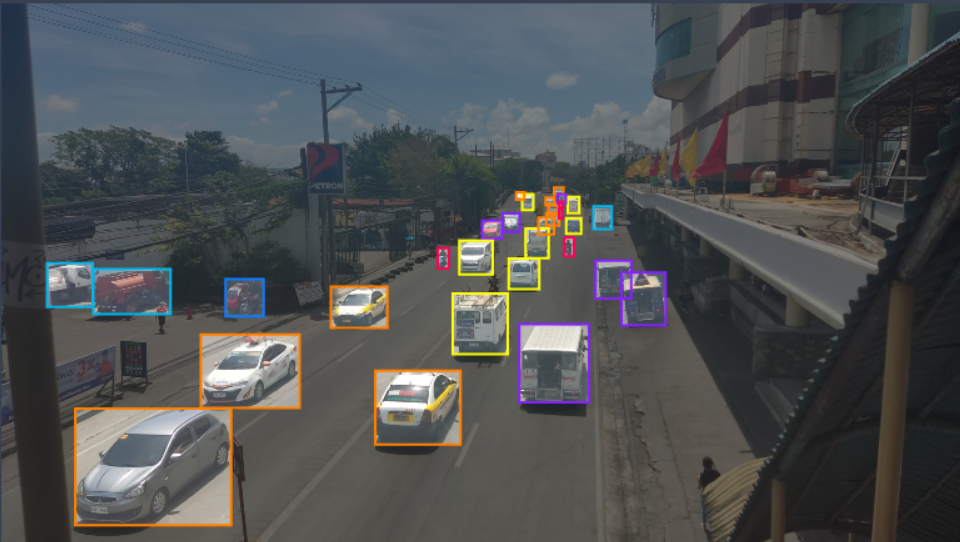
\includegraphics[width=\linewidth]{full_img_anno.png}
	\caption{Object Detection Prototype used for Traffic recorded in street view}
	\label{fig:full_img_anno}
\end{figure}

Figure \ref{fig:cropped_anno} uses a vehicle cropping method. In this specific example, the researchers needed more data of the tricycle. Hence, samples of tricycles over different images/frames from videos were cropped before being uploaded to the Roboflow annotation tool. 

\begin{figure}[h!]
	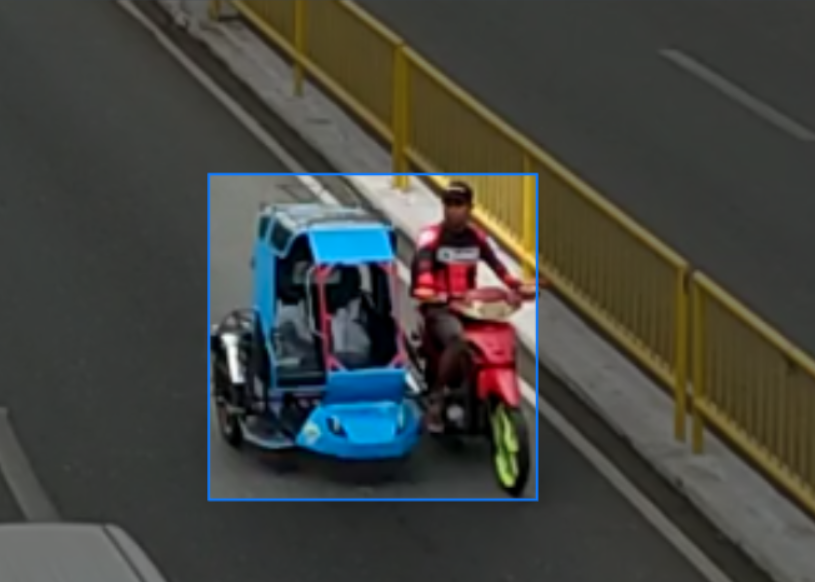
\includegraphics[width=\linewidth]{cropped_anno.png}
	\caption{Object Detection Prototype used for Traffic recorded in street view}
	\label{fig:cropped_anno}
\end{figure}

\newpage

\subsection {Training and Performance Testing}

The training data will be separated into different classes and is also the bases of classification for the training: cars, jeepneys, motorcycles, tricycles, trucks, and utility vehicles. The training will be done using the “train.py” in the YOLOv5 repository with the following line of code used in the Google Colab Notebook for training the data:


\lstset{language=python,
	aboveskip=3mm,
	belowskip=3mm,
	showstringspaces=false,
	columns=flexible,
	basicstyle={\small\ttfamily},
	numbers=none,
	breaklines=true,
	breakatwhitespace=true,
	tabsize=3
}
\begin{lstlisting}[frame=single]
	!git clone https://github.com/ultralytics/yolov5
	%cd yolov5
	%pip install -qr requirements.txt
	import torch
	import utils
	display = utils.notebook_init()
	
	
\end{lstlisting}

The data was trained with 16 batches and 300 epochs. These are reflected by the following terminal command for training.

\newpage


\begin{lstlisting}[frame=single]
	!python /content/yolov5/train.py --batch 16 --epochs 300 --data /content/drive/MyDrive/College/SP/data/data.yaml --weights yolov5m.pt --cache
	
\end{lstlisting}


The “/content/drive/MyDrive/College/SP/data/data.yaml” is the yaml file that contains the information about the different classes in the dataset. Below is an example of data.yaml.


\begin{lstlisting}[frame=single]
	
	train: ../train/images
	val: ../valid/images
	test: ../test/images
	
	nc: 6
	names: ['Car', 'Jeepney', 'Motorcycle', 'Tricycle', 'Truck', 'Utility Vehicle']
	
	roboflow:
	workspace: special-project
	project: sp-cmsc198.1
	version: 3
	license: CC BY 4.0
	url: https://universe.roboflow.com/special-project/sp-cmsc198.1/dataset/3
	
	
\end{lstlisting}

The file contains the directory to the train, validation, and testing data as well as other important information such as the number of objects and their names that is needed by”train.py”. 

For performance testing, there are visualization tools available to visualize the performance of the model after training. If little to no improvement is being done by subsequent iterations on the performance parameters the training will be interrupted. To benchmark the performance of the training, the custom model will be be compared against manual counting of vehicles.

\newpage
\section {Model Applictation}
The program detect.py will be run to detect objects from an external device or video file using the trained model. When detect.py is run it will start to list the objects it detects. An average emission of each vehicle type will be used. The study from \cite{rito_lopez_biona_2021} provides a table that quantifies the emission factors of energy consumption of multiple vehicle types, 6 of which are to be used in this study. The emission data from the study will be utilized for the application.The table below shows the grams of emissions per kilometer.
The averages of the vehicles’ $PM_{2.5}$ emissions  at a given time will be displayed in a real-time chart and will be periodically updated as vehicles enter and leave the camera’s or video’s line of sight. 

\begin{table}[ht]   %t means place on top, replace with b if you want to place at the bottom
\centering
\caption{Emission factors per vehicle type ($g_{emissions}/km$)} \vspace{0.25em}
\begin{tabular}{|p{2in}|c|c|c|c|} \hline
\centering Vehicle Type & $PM_{2.5}$ & \ch{CH4} & \ch{N2O} & \ch{CO2} \\ \hline
Tricycle   & 0.0562   & 4.0906 & 0.0021 &  66.8747\\ \hline
Motorcycle& 0.0336  &2.3022   & 0.0015 & 60.0983\\ \hline
Jeepney &0.8466&0.2357  &0.0316	& 668.7415\\ \hline
Car & 0.0221 & 0.7408  & 0.0099  & 109.8958\\ \hline
Utility & 0.1430 & 0.3538 & 0.0063 & 92.4039\\ \hline
Light Truck & 0.7519 & 0.3648 & 0.0226 & 842.0852\\ \hline

\end{tabular}
\label{tab:emission}
\end{table}

\subsubsection{Calculating the $PM_{2.5}$ Emission Estimate}

The system, after assigning values to each vehicle, shall calculate the vehicles’  $PM_{2.5}$ emissions using the following equation:
\[\frac{\sum\text{(total count of vehicle x * vehicle x's assigned $PM_{2.5}$ value)}}{\text{Total vehicles detected}} \]
The total count of the vehicle X is multiplied to its assigned  $PM_{2.5}$ value. The sum of the product of every vehicle is then divided by the total number of detected vehicles on the frame to get the average. This results in the estimated  $PM_{2.5}$ value being produced from vehicles in a current frame.


\section{System Architecture}

A separate system for inference was made to allow the program to count the number of vehicles and approximate emissions. The available program for detection (detect.py) was not used because it was meant to run for general cases and not for videos and webcam footage of vehicles specifically as indicated in the github page for YOLOv5 (https://github.com/ultralytics/yolov5). 

\begin{figure}[h!]
	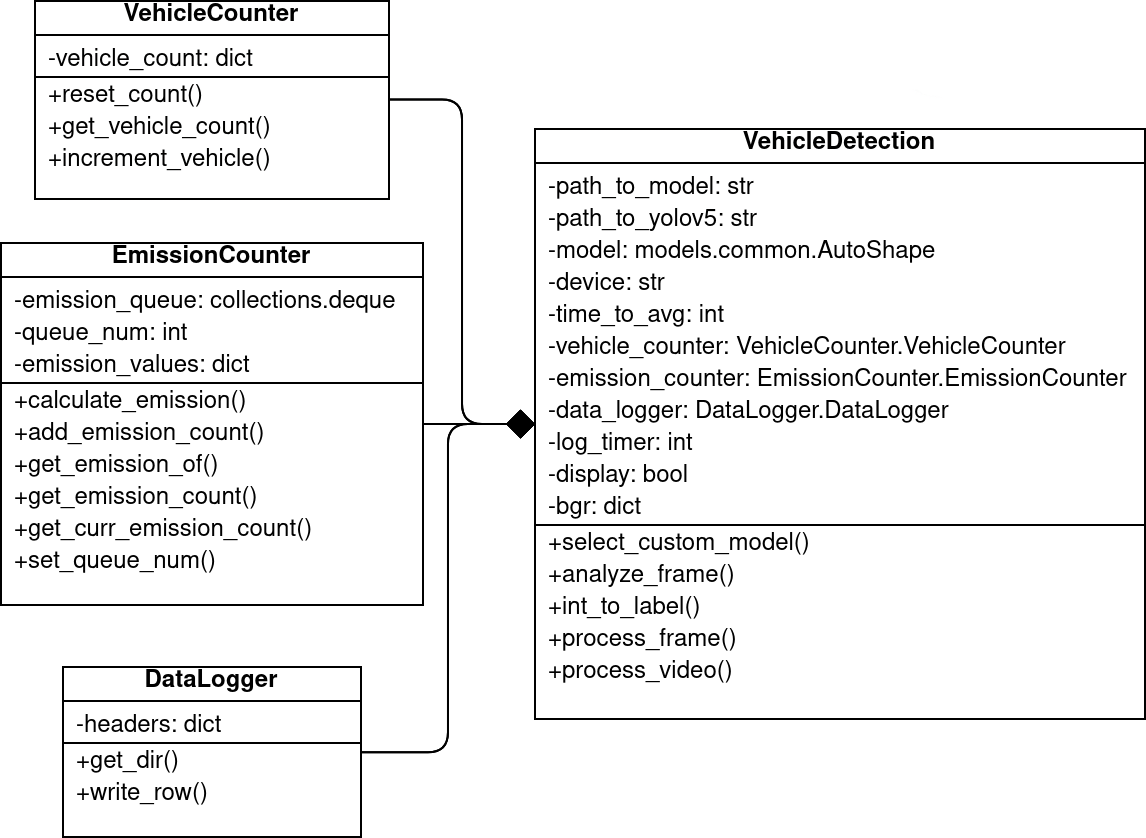
\includegraphics[width=\linewidth]{system_uml.png}
	\caption{Object Detection Prototype used for Traffic recorded in street view}
	\label{fig:system_uml}
\end{figure}

As shown in Figure \ref{fig:system_uml} The system contains four classes. The VehicleDetection class is the class that makes objects for detecting vehicles and counting emissions, and this class utilizes three other classes: VehicleCounter, EmissionCounter, and DataLogger. This composition was done so that one class only has one role. The VehicleCounter class serves as a click counter for different vehicles and was used to count vehicles in a single frame. The EmissionCounter class stores the emission estimate in a double-ended queue so that the average emissions for a number of frames can be calculated. The DataLogger class logs the data into an external CSV file. 

The VehicleDetection class is responsible for analyzing each frame of a video, detecting the objects from the frame, and incorporating the three classes to count vehicles from a video, averaging the PM2.5, and exporting the data into a CSV file.

%
%\section{Calendar of Activities}
%
%Table \ref{tab:timetableactivities} shows a Gantt chart of the activities for the development of Hazy.  Each bullet represents approximately
%one week worth of activity.
%
%%
%%  the following commands will be used for filling up the bullets in the Gantt chart
%%
%\newcommand{\weekone}{\textbullet}
%\newcommand{\weektwo}{\textbullet \textbullet}
%\newcommand{\weekthree}{\textbullet \textbullet \textbullet}
%\newcommand{\weekfour}{\textbullet \textbullet \textbullet \textbullet}
%
%%
%%  alternative to bullet is a star 
%%
%\begin{comment}
%   \newcommand{\weekone}{$\star$}
%   \newcommand{\weektwo}{$\star \star$}
%   \newcommand{\weekthree}{$\star \star \star$}
%   \newcommand{\weekfour}{$\star \star \star \star$ }
%\end{comment}
%
%
%%
%\begin{table}[ht]   %t means place on top, replace with b if you want to place at the bottom
%\centering
%\caption{Timetable of Activities} \vspace{0.25em}
%\begin{tabular}{|p{2in}|c|c|c|c|c|c|c|c|c|c|} \hline
%\centering Activities  & Sept  & Oct & Nov & Dec & Jan & Feb & Mar & April & May & June\\ \hline
%Finding and Choosing Final Topic      & ~~~\weektwo &  &  &  &  &  & &&& \\ \hline
%Review of Related Literature &   & \weekfour & \weekfour &  &  &  & & ~~~\weekone& \weekone~~~ & \\ \hline
%Identifying Problem Statement     &  ~~~\weektwo &  \weekone~~~  &  & &  &  &  &&&\\ \hline
%Formation of Possible Solution    &   & ~~~\weektwo  &  \weekone~~~ &  & & & &&&  \\ \hline
%Constructing the Methodology     &   &  &   ~~~\weektwo & \weekthree ~~ & &  & &&& \\ \hline
%
%Documentation & ~~~\weektwo  & \weekfour & \weekfour &\weekone ~~& & ~~~\weektwo &  & ~~~\weektwo & \weekone~~~ & ~~~\\ \hline
%Model Training   &  &  &  & & & & \weekone~~~  & ~~~\weektwo & \weekone~~~  & \\ \hline
%Data Gathering & & & & & &\weekfour&\weekfour& \weekfour & &~~~  \\ \hline
%Testing     &   &  &  & \weekthree ~~ & &  & ~\weekone~ & ~~~\weekone & \weekone~~~ &  \\ \hline
%Interpretation of Results     &   &  &  & \weekthree ~~ & &  & &~~~\weekone& \weekone~~~ & \\ \hline
%
%\end{tabular}
%\label{tab:timetableactivities}
%\end{table}

